\documentclass[letterpaper]{article}
\usepackage{import}{\tiny }
\usepackage{standalone}
\usepackage[english]{babel}
\usepackage[a4paper]{geometry}
\usepackage[utf8]{inputenc}
\usepackage{float}
\usepackage{amsmath}
\usepackage{amssymb}
\usepackage{amsthm}
%\usepackage{cool} %seems cool. has bugs. conflicts with own derivative commands (below)
\usepackage{enumitem}
\usepackage{fancyhdr}
\usepackage{multirow}
\usepackage{booktabs}
\usepackage{subfiles}
\usepackage{siunitx}
\usepackage{graphicx}
\usepackage{caption}
\usepackage{subcaption}
\usepackage{hyperref}
\usepackage{appendix}
\usepackage{rotating}
\pagestyle{fancy}

%Packages and settings for code formatting
\usepackage{color}
\definecolor{code_keywords}   {rgb}{0,0,0} %blue={0.13,0.13,0.75}
\definecolor{code_comments}   {rgb}{0.17,0.57,0.17}
\definecolor{code_linenumbers}{rgb}{0.5,0.5,0.5}
\definecolor{code_strings}    {rgb}{0,0,0} %red={0.5,0,0}
\usepackage{listings}
\lstset{
	language		 = Matlab,
	basicstyle		 = \footnotesize,
	commentstyle	 = \color{code_comments},
	keywordstyle	 = \bfseries\color{code_keywords},
	stringstyle		 = \color{code_strings},
	numberstyle		 = \tiny\color{code_linenumbers},
	frame			 = none,
	keepspaces		 = true,
	numbers			 = left,
	numbersep		 = 5pt,
	showspaces		 = false,
	showstringspaces = false,
	showtabs		 = false,
	stepnumber		 = 1,
	tabsize			 = 4,
}


\lfoot{} % Controls the left corner of the footer
\cfoot{} % Controls the center of the footer
\rfoot{page~\thepage} % Controls the right corner of the footer
\renewcommand{\headrulewidth}{0.4pt}
\renewcommand{\footrulewidth}{0.4pt}

%Specify table columns' width
\newcolumntype{L}[1]{>{\raggedright\arraybackslash}p{#1}}
\newcolumntype{C}[1]{>{\centering\arraybackslash}p{#1}}
\newcolumntype{R}[1]{>{\raggedleft\arraybackslash}p{#1}}


\newcommand{\todo}[1]{\textcolor{red}{\textbf{[TODO]}~#1}}

\newcommand{\imp}{\Rightarrow} %mathematical "implies"
\newcommand{\Imp}{\quad\imp\quad} %...with spacing


\author{Giovanni Bologni (\todo{?}) and Wouther Bons (4092716)}
\date{\today}
\title{EE4389\\Modeling and Data Analysis in Complex Networks\\Assignment}
\lhead{EE4389 Complex Networks Assignment} % Controls the left corner of the header
\chead{} % Controls the center of the header
\rhead{Giovanni Bologni and Wouther Bons} % Controls the right corner of the header

\begin{document}

\maketitle

\subsection*{Introduction}
When measurements are performed on a network, the resulting dataset can be analysed to quantify properties of the underlying network. In this assignment a dataset of face-to-face contact data of highschool students\footnote{R. Mastrandrea, J. Fournet, A. Barrat, Contact patterns in a high school: a comparison between data collected using wearable sensors, contact diaries and friendship surveys. PLoS ONE 10(9): e0136497 (2015)} is analysed.

This data not only includes contact information at a certain time, but also how contact changes over time; every measurement specifies which two students have had contact and at which time this occured. Students will be modeled as nodes in a graph and contact between students as edges. Each edge will also be labeled with the timestamp at which the contact it represents was made.

To begin with, this data will be aggregated over all time to analyse the topology of the resulting aggregated network. Secondly, the time of measurement will be taken into consideration. Several metrics will be used to analyse which nodes are most influential when information spreads across this temporal network. Lastly, temporal features of the network will be altered to inspect their influence on the information spreading process.

\subsection*{Part A: Topological features of the aggregated network}
The aggregated graph \(G\) is constructed by connecting any two nodes by an (unweighted) edge if the nodes make contact with eachother at least once in the \(T=7375\) timesteps available.

\(G\) has \(N=327\) nodes and \(L=5818\) links. The link density is computed as
\begin{align*}
p = \frac{E[L]}{L_{max}} = \frac{L}{N(N-1)/2} = 0.1092
\end{align*}

Several metrics inspect the degree of nodes in the network, of which an insightful one is the degree distribution (fig.~\ref{fig:degree_distribution}). It can be seen that this distribution resembles a Poisson distribution. This suggests that an Erdös-Renyi (ER) graph model would be well suited to model the face-to-face contact network. In contrast, a scale-free graph model would be a bad choice of model because scale-free graphs show a linear distribution when viewed on a log-log scale and this is absolutely not the case (fig.~\ref{fig:degree_distribution_loglog}).

The average and variance of the degree are \(E[D]=35.58\) and \(Var[D]=182.2\), respectively. The degree assortativity (\(\rho_D=0.03318\)) is defined as the (linear) correlation coefficient between the degrees of nodes, so a value of almost zero means the degrees of nodes are not correlated at all. This means that the creation of new links is not influenced by existing links; another argument for using the ER graph model, where edges are created with independent probabilities (and are therefore uncorrelated).

\begin{figure}
    \centering
    \begin{subfigure}[b]{0.45\textwidth}
        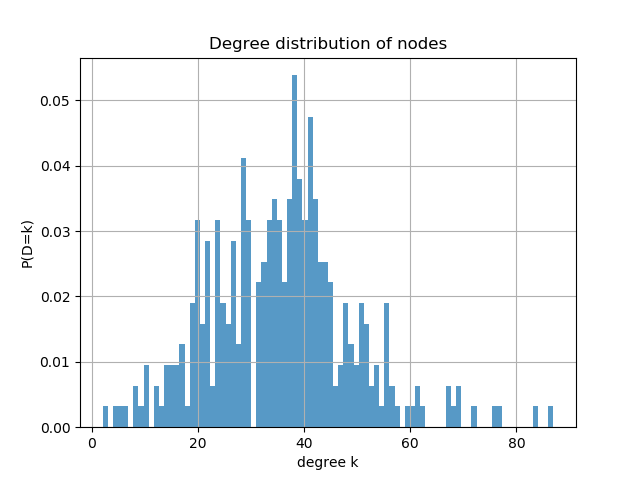
\includegraphics[width=\textwidth]{img/degree_distribution.png}
        \caption{Linear scale}
	    \label{fig:degree_distribution_linlin}
    \end{subfigure}
    ~ % spacing
    \begin{subfigure}[b]{0.45\textwidth}
        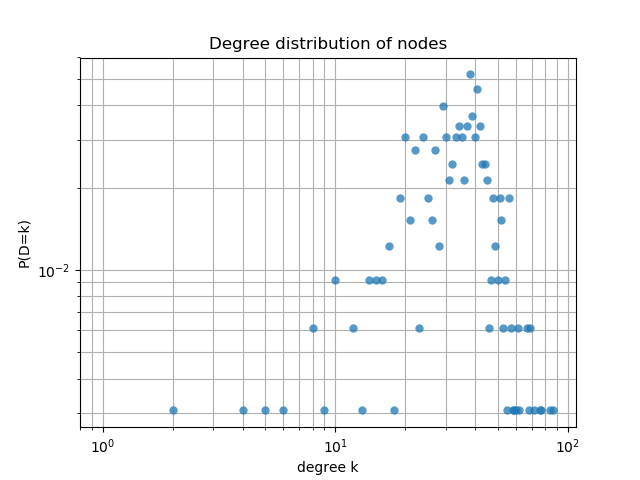
\includegraphics[width=\textwidth]{img/degree_distribution_loglog.png}
        \caption{Log scale}
	    \label{fig:degree_distribution_loglog}
    \end{subfigure}
    \caption{Degree distribution of nodes in the aggregated graph.}
    \label{fig:degree_distribution}
\end{figure}

Furthermore, it is interesting to check whether the network exhibits the small-world property, i.e. nodes are not very clustered but can still reach other nodes in relatively few hops. Using the clustering coefficient (\(C=0.5035\)) and average hopcount (\(E[H]=2.159\)) normalized by that of the regular graph results in the following metrics: \todo{suspicious that they're larger than one...}
\begin{align*}
C/C(0) = 4.681\\
E[H]/E[H](0) = 1.132
\end{align*}
Because the (normalized) clustering coefficient is several times higher than the average hopcount, the network exhibits the small-world property. \todo{C\(>\)E[H] shows from the graph on the slides, but I thought the clustering had to be lower, not higher?!}

\todo{L proportional to log N for small-world networks (plot over time) better test for small-world property?}

Comparing the average hopcount (\(E[H]=2.159\)) with the diameter of the graph (\(H_{max}=4\)) we see that there is not a lot of variance in hopcounts of shortest paths between nodes; the diameter (the worst-case hopcount of shortest paths) is close to the graph's efficiency (the average hopcount). This again points to the small-world property.

Lastly, some spectral metrics of the aggregated graph are considered. The spectral radius is calculated as the largest eigenvalue of the adjacency matrix \(\lambda_1=41.23\). The algebraic connectivity is the second smallest eigenvalue of not the adjacency but the Laplacian matrix, \(a=\mu_{N-1}=1.930\). \todo{is this a lot or not? perhaps compare with upper bound 1/nD where n is nodes in complete graph?}


\subsection*{Part B: Information spreading on a temporal network}
\todo{}


\subsection*{Part C: Influence of temporal network features on information spreading}
\todo{}


\subsection*{Conclusion}
\todo{}



%begin{table}[ht!]
%	\centering
%	\begin{tabular}{@{} L{9em} *{10}{R{1.75em}} @{}}
%		\toprule
%		instruction						& 1		& 2		& 3		& 4		& 5		& 6		& 7		& 8		& 9		& 10	\\
%		\midrule
%		\texttt{lw \$r2, 0(\$r1)}		& IF	& ID	& EX	& \underline{MEM}	& WB	& 		& 		& 		& 		& 		\\
%										&		& NOP	& NOP	& NOP	& NOP	& NOP	& 		& 		& 		& 		\\
%		\texttt{and \$r1, \$r2, \$r1}	& 		& 		& IF	& ID	& \underline{EX}	& MEM	& WB	& 		& 		& 		\\
%		\texttt{lw \$r3, 0(\$r2)}		& 		& 		& 		& IF	& ID	& EX	& MEM	& WB	& 		& 		\\
%		\texttt{lw \$r1, 0(\$r1)}		& 		& 		& 		& 		& IF	& ID	& EX	& MEM	& WB	& 		\\
%		\texttt{sw \$r1, 0(\$r2)}		& 		& 		& 		& 		& 		& IF	& ID	& EX	& MEM	& WB	\\
%		\bottomrule
%	\end{tabular}
%	\caption{Pipeline execution diagram for the code in the first column when the datapath does have a forwarding unit as well as hazard detection. Underlined stages indicate a forwarding connection between these stages. The total execution time is 10 clock cycles.}
%	\label{tab:PipelineTableD}
%end{table}


\end{document}
